\chapter{Project Planning \& Management} \label{Chapter:Project Planning & Management}


\section{Team Management}
\subsection{Project Management Plan and Technique}
Prior to the start-up of the project, the team had a meeting to introduce and get to know each other, before assigning the role of Project Manager and Vice President (VP). As the discussion goes on, the project was break down into few main components, known as a Work Breakdown Structure (WBS), which turned the overwhelming works into manageable pieces. An individual skills assessment has been created within the team so that the components can be divided to each of the member depending on their ability, knowledge and the comfortability to handle the task. Together with the official deadlines released by the University, Gantt chart, a visual timeline across the life cycle of a project is made, with start and estimated end dates for each of the individual tasks set up. Over the time throughout the project, Gantt Chart often was modified or updated, to include more detailed tasks as a subsection in the main huge components. With Gantt chart, the scheduled works that have been planned initially can be compared with the actual timelines of the project, keeping track with the goals.

A Kanban management method also being used, using a collaboration tool Trello to organize and keeping track, where any small tasks or deadline were recorded into boards, specifying person-in-charge, what is being worked on, and the progress. Besides, to ensure the quality of the project, weekly meetings of at most three are being scheduled. 
\begin{itemize}
    \item Monday – unofficial meeting with the team members, mainly to discuss to progress made within the past week and preparation to make for the official meeting on Tuesday.
    \item Tuesday – official meeting with InterDigital partner to discuss on the project especially on the progress and development.
    \item Thursday – meeting with supervisor to update the progress made on respective week, discuss anything matter about the project.
\end{itemize}

All the discussion, idea for development, progress and on-going task were kept in minute meetings by project manager. While a small list based on weekly sprint approach, where on-going, priority and completed tasks are shown, was done as well after the meeting and attached together in the email thread that include all the team members, supervisor and our InterDigital partner. As the project goes on, a hard deadline has been decided in order to motivate and push the team members on working and developing the product as much as we can before focusing solely on the report writing. 

A skeleton or content draft was made by VP as a guide to assist the writing flow. The write up was planned to be about two weeks, before sending it over to the supervisor and InterDigital partner for proof-reading, getting advises and critics. Based on the involvement during the project, each of the team members are responsible to write their research, results and discussion on the part they were assigned to before. Depending on the progress made, the remaining works were divided fairly, taking into consideration on the time availability of the person, making sure everyone works fairly at the same pace and same workloads. Throughout the writing period, a daily meeting was made at the end of the day to keep track of everyone’s work and progress, motivating each other for the last push of the project.

\subsection{Division of Responsibility}
Below is the roles and responsibilities assigned to each of the members in order to get the project to progress smoothly. 

\textbf{Project Manager - }
Individual responsible to deliver the project by leading and manages project team on a day-to-day basis, communicating with each of the team members regarding the tasks assigned, checking the progress. Project manager also has an important role in interfacing between the team, supervisor and business partner from the respective company collaborated with. Specific responsibilities of project manager:
\begin{itemize}
    \item Set up the communication medium for the members to discuss the progression of tasks.
    \item Scheduling meetings between the team members, supervisors and client from the company.
    \item Keeping the minute meetings.
    \item Summarize the discussion made during the meetings, next tasks assigned for each member for the record of supervisor and the client, through email thread.
    \item Monitor overall progress of the project.
\end{itemize}

\textbf{Vice President (VP) of Assessment - }
A role where the person in charge needs to review the criteria needed in the assessment, remind the deadlines of each submission and responsible as a representative from the team to do the submissions.

\textbf{Project Team Members - }
Under the supervision and direction of the project manager, the team members are responsible for carrying work detailed laid out in the programme plan. Breaking down the tasks of the project which is to establish the end-to-end (E2E) wireless telemetry pipeline using latest cloud technologies to accelerate wireless system research for Industry 4.0 use cases, there are five main components of the tasks divided.

\begin{table}[ht]
\centering
\begin{tabular}{ |c|p{9cm}|c| } 
 \hline
 Index & Main Task & Person-in-Charge\\ 
  \hline
1 & Design a telemetry service for WiFi/5G NR that is producing wireless data & Akshay \\ 
  \hline
2 & Set up edge nodes with deployed edge applications & Syuhada, Anurag \\ 
  \hline
3 & Create AWS data lake for stream/batch processing & Anurag \\ 
  \hline
4 & Select AWS ML tools that allows model training and model deployment & Eu Jin \\ 
  \hline
5 & Create OTT application & All \\ 

 \hline
\end{tabular}
\caption{Task assignment and the person-in-charge. }
\label{table:task_management}
\end{table}

These tasks were assigned based on each of the member skills, knowledge and comfortability to handle the task before merging the individual work into one whole system in the final stage. Since there are four people in the group when there are five main components, the sequence of the workflow was being prioritized first in order to make the system work.

\subsection{Meetings and Notes}
Discussion made in every meeting scheduled was kept into minute meetings (referred in Appendix). While a list of tasks using weekly sprint-based approach is produced after each meeting, where on-going, priority and completed tasks are shown in Figure \ref{fig:task_list}. 

\begin{figure}[ht]
    \centering
    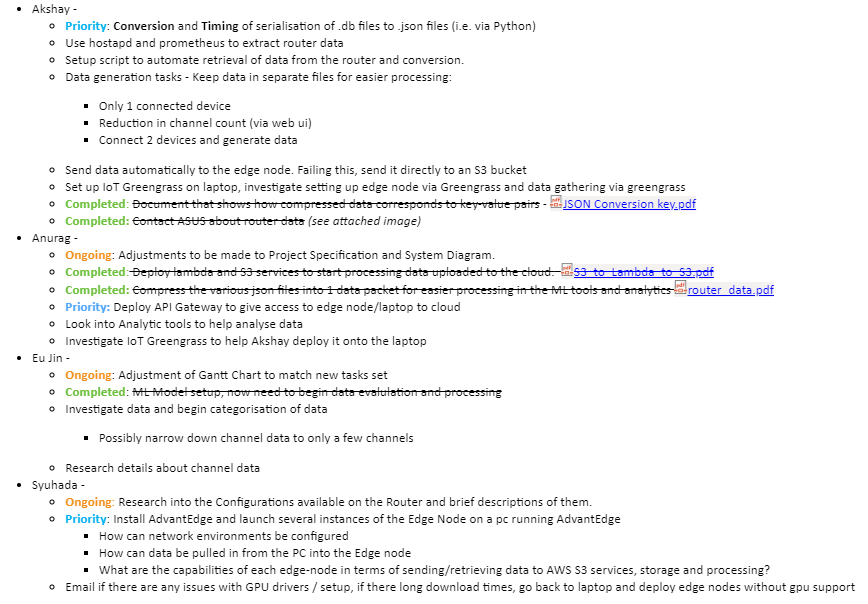
\includegraphics[width=1\linewidth]{images/Task_list.png}
    \caption{Weekly sprint-based list that includes the on-going task, priority and completed tasks assigned for each team members.}
    \label{fig:task_list}
\end{figure}

\subsection{Communication within the Team}
Project teams can effectively communicate through the weekly meeting or the formal project discussion meeting with the company’s representative or supervisor. Information can be shared through anything in the form of written notes to complex extension of files. As part of the responsibility, project manager has identified the method and approved way of communicating. These includes:
\begin{table}[]
    \centering
    \begin{tabular}{p{14cm}l}
      \hline
      \textbf{Microsoft Teams}  \\
      \hline 
         \begin{itemize}
             \item Mainly used for online meetings to discuss the progress made, issue encountered and idea for improvement. Make it easier to communicate especially screen can be shared by individual participant.
             \item Information, data or documents can be shared in the folders for everyone in the group to access and download. Any modification can be made online on the documents.
             \item Base for the offline discussion on the general timeline.
         \end{itemize} \\
         \hline
      \textbf{Outlooks (email)}  \\
            \hline 
         \begin{itemize}
             \item The medium used to communicate with the supervisor (university) and the client (company’s representative).
             \item To update and summarize the meetings’ contents, as well as the status report (list of team members’ progress and ongoing tasks).
             \item The reminder for the scheduled meetings.
         \end{itemize} \\
         \hline
    \end{tabular}
    \caption{Communication medium used in the project between the team members, supervisor and InterDigtal Partner.}
    \label{tab:communication}
\end{table}

\section{Technical Approach}
\subsection{Gantt Chart}

\section{Risk Assessment}
